\themaG
\graphicspath{{../Ch10_Droites_perpendiculaires_paralleles/Images/}}

\chapter{Droites\\perpendiculaires\\et parallèles}
\label{C15}

%%%%%%%%%%%%%%%%%%%%%%%%%%%%%%%%%%%%%%%%%%
\begin{prerequis}[Connaissances et compétences abordées]
   \begin{itemize}
      \item Tracer avec l’équerre la droite perpendiculaire à une droite donnée passant par un point donné.
      \item Tracer avec la règle et l’équerre la droite parallèle à une droite donnée passant par un point donné.
      \item Déterminer le plus court chemin entre un point et une droite.
      \item Distance entre un point et une droite.
   \end{itemize}
\end{prerequis}

\vfill

\begin{debat}[Débat : un YouTubeur matheux !] 
   {\bf Yvan Monka} est professeur de mathématiques dans l'académie de Strasbourg : il dispose d'un site internet {\it m@ths et tiques} avec de nombreux cours et exercices de la sixième à la terminale et d'une chaîne YouTube comportant près de 1\,500 vidéos, à consommer sans modération !!! \\
   \begin{center}
      
\includegraphics[width=5cm]{Monka}
   \end{center}
   \bigskip
   \begin{cadre}[B2][F4]
      \begin{center}
         Vidéo : \href{https://www.youtube.com/watch?v=tUzoATZrAmc}{\bf Mesurer la distance d'un point à une droite}, chaîne YouTube d'{\it Yvan Monka}.
      \end{center}
   \end{cadre}
\end{debat}

\vfill

\textcolor{PartieGeometrie}{\sffamily\bfseries Cahier de compétences} : chapitre 7, exercices 2 à 15 ; 23 ; 24 ; 26 ; 29.


%%%%%%%%%%%%%%%%%%%%%%%%%%%%%%%%%%%%
%%%%%%%%%%%%%%%%%%%%%%%%%%%%%%%%%%%%
\activites

   \begin{activite}[La carte au trésor]
      {\bf Objectifs :} tracer une droite parallèle ; une droite perpendiculaire ; se repérer sur un plan ; suivre un programme.
      \begin{QCM}
         Un lutin trouve un jour un parchemin en sortant de sa maison.
Ce parchemin est en fait la carte d’un trésor caché. Voici ce qui est écrit dessus :
         \begin{center}
            \fbox{\begin{minipage}{12cm}
               \og {\it À partir de cet endroit, fait 550 m perpendiculairement à la Route de la baie, vers la mer. \\
               Ensuite, fait 900 m parallèlement à la route de la ville, vers le nord-ouest. \\
               Poursuis ta route parallèlement à la route de la baie en faisant 750 m vers le sud-est. \\
               Enfin, perpendiculairement à la route de la ville vers le nord-est, fait 270 m. \\
               Tu trouveras ainsi le trésor.} \fg
            \end{minipage}}
         \end{center}
         Où se trouve le trésor ? Faire les tracés nécessaires sur la feuille. \\ [3mm]
            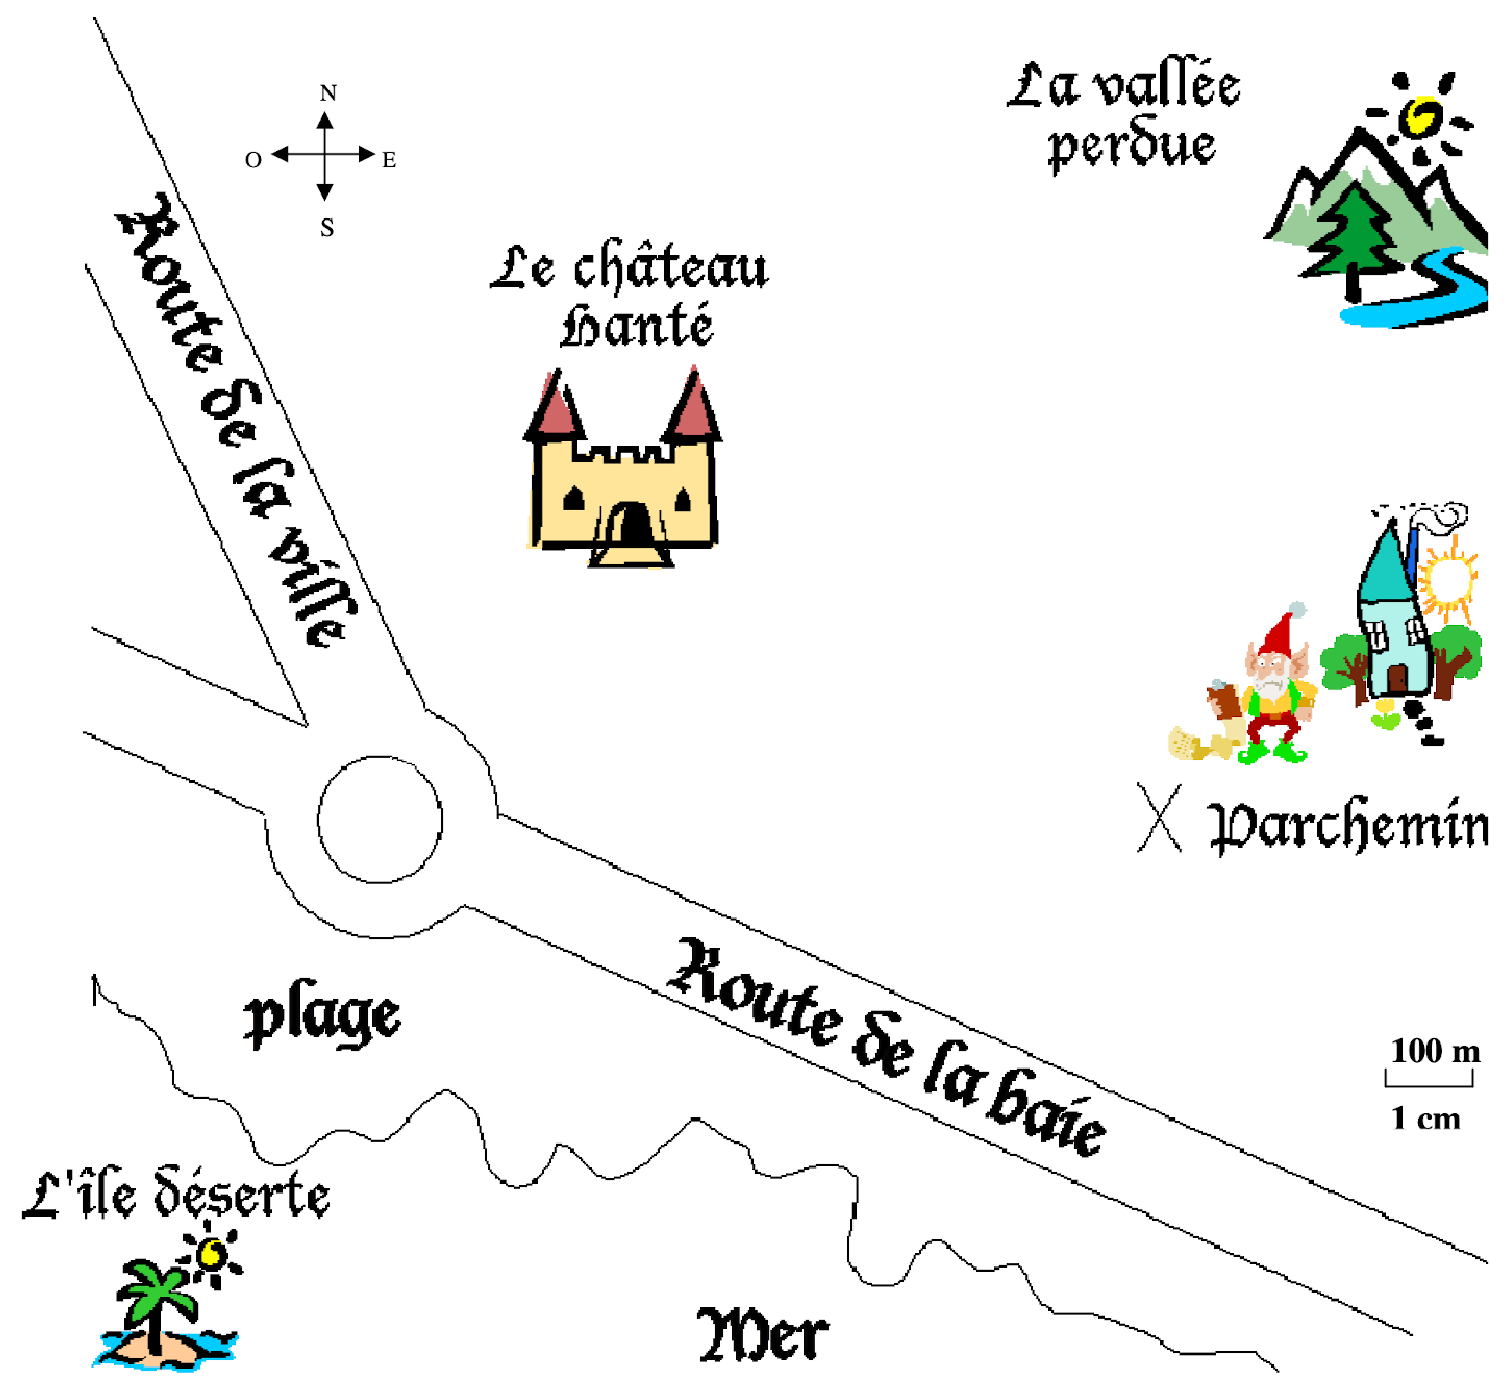
\includegraphics[width=16.8cm]{tresor}
      \end{QCM}
\end{activite}


%%%%%%%%%%%%%%%%%%%%%%%%%%%%%%%%
%%%%%%%%%%%%%%%%%%%%%%%%%%%%%%%%
\cours 

%%%%%%%%%%%%%%%%% I %%%%%%%%%%%%%%%
\section{Construction de droites perpendiculaires et parallèles}

Pour construire des droites perpendiculaires et parallèles à une droite passant par un point, on peut utiliser le quadrillage de sa feuille ou une règle et une équerre.

\begin{methode}[Construction d'une perpendiculaire avec une équerre]
   Pour construire la perpendiculaire $(d)$ à une droite $(D)$ passant par un point $A$, on place la règle le long de la droite $(D)$, puis on place un bord de l'équerre (contenant l'angle droit) contre la règle avec l'angle droit au niveau du point $A$ et on trace la droite $(d)$.
   \exercice
      \begin{pspicture}(0,-0.5)(3.5,2.6)
         \psline(0,0)(4,1)
         \psdot[dotstyle=+](1,0.25)
         \rput(0.7,0.45){$A$}
         \rput(3.6,1.2){$(D)$}
      \end{pspicture} 
   \correction
      \qquad
      \begin{pspicture}(0,-0.5)(3.5,2.6)
         \psline(0,0)(4,1)
         \psdot[dotstyle=+](1,0.25)
         \rput(0.7,0.45){$A$}
         \equerre{1}{0.25}{14}{1}
         \regle{0}{-0.29}{14}{1}
         \rput(3.6,1.2){$(D)$}
      \end{pspicture}      
      \qquad
      \begin{pspicture}(0,-0.5)(3.5,2.6)
         \psline(0,0)(4,1)
         \psdot[dotstyle=+](1,0.25)
         \rput(0.7,0.45){$A$}
         \psline[linecolor=A1,linewidth=0.05](1.135,-0.3)(0.34,2.9)
         \equerre{1.02}{0.28}{14}{1}
         \rput(3.6,1.2){$(D)$}
         \rput(0.8,2.7){\textcolor{A1}{$(d)$}}
      \end{pspicture}
\end{methode}

\medskip

\begin{methode}[Construction d'une parallèle à la règle et à l'équerre]
   Pour tracer la parallèle $(\Delta)$ à $(D)$ passant par $B$, on trace la perpendiculaire $(d)$ à $(D)$ passant par $B$, puis on trace la perpendiculaire $(\Delta)$ à $(d)$ passant par $B$.
   \exercice
      \begin{pspicture}(-0.5,-0.4)(3.5,3)
         \psline(0,0)(4,1)
         \psdot[dotstyle=+](0.65,1.69)
         \rput(0.55,1.45){$B$}
         \rput(3.6,1.2){$(D)$}
      \end{pspicture}  
   \correction   
      \begin{pspicture}(-0.3,-0.4)(3.5,3)
         \psline(0,0)(4,1)
         \psdot[dotstyle=+](0.65,1.69)
         \rput(0.55,1.45){$B$}
         \psline[linecolor=A1,linewidth=0.05](1.135,-0.3)(0.34,2.9)
         \equerre{1.02}{0.28}{14}{1}
         \regle{0}{-0.25}{14}{1}
         \rput(3.6,1.2){$(D)$}
         \rput(0.6,2.5){\textcolor{A1}{$(d)$}}
      \end{pspicture} 
      \begin{pspicture}(-1,-0.4)(3.5,3)
         \psline(0,0)(4,1)
         \psdot[dotstyle=+](0.65,1.69)
         \rput(0.55,1.45){$B$}
         \psline[linecolor=B2,linewidth=0.05](-0.2,1.5)(3.8,2.5)
          \equerre{0.68}{1.68}{-76}{1}
         \psline[linecolor=A1,linewidth=0.05](1.135,-0.3)(0.34,2.9)
         \rput(3.6,1.2){$(D)$}
         \rput(0.8,2.5){\textcolor{A1}{$(d)$}}
         \rput(3.5,2.85){\textcolor{B1}{$(\Delta)$}}
         \regle{0.25}{2}{-76}{1}
      \end{pspicture} 
\end{methode}
   
\begin{remarque}
   deux droites perpendiculaires à une même droite sont parallèles.
\end{remarque}


%%%%%%%%%%%%%%%%%%%%%%%%%%%%%%%%%%%%%%%%%
\section{Distance d'un point à une droite}

\begin{minipage}{11cm}
   \begin{definition}
      La distance d'un point $A$ à une droite $(d)$ est la plus courte distance séparant le point A d'un point de $(d)$.
   \end{definition}
   \smallskip
   \begin{propriete}
      La distance d'un point $A$ à une droite $(d)$ est égale à la longueur du segment [AH] où H est le pied de la perpendiculaire à $(d)$ passant par $A$.
   \end{propriete}
\end{minipage}
\begin{minipage}{7cm}
   \begin{pspicture}(1.5,1.5)(6,6)
      \pstGeonode[PointSymbol=+,PosAngle={90,-45}](1,5){A}(4,4){P}(2,2){N}(5,5){Q}(3,3){H}
      \pstLineAB[nodesep=-10mm]{N}{Q}
      \pstLineAB[linecolor=A1]{A}{N}
      \pstLineAB[linecolor=B1]{A}{H}
      \pstLineAB[linecolor=A1]{A}{P}
      \pstLineAB[linecolor=A1]{A}{Q}
      \pstRightAngle[linecolor=B1]{Q}{H}{A}
      \rput(5.5,3){\textcolor{B1}{distance de $A$ à $(d)$ : AH}}
      \rput(6,6){$(d)$} 
   \end{pspicture}
\end{minipage}


%%%%%%%%%%%%%%%%%%%%%%%%%%%%%%%%%%%%%%%%%%
\exercicesbase

\begin{colonne*exercice}

\serie{Tracé de droites}

\begin{exercice}
   Sur ces trois figures, tracer en rouge la droite parallèle à la droite $(d)$ passant par $A$ et en vert la droite perpendiculaire à la droite $(d)$ passant par $B$.
   \begin{center}
      \psset{unit=0.68}
      \begin{pspicture}(11,9)
         \psgrid[subgriddiv=1,griddots=5,gridlabels=0](0,0)(11,9)
         \pstGeonode[PointSymbol=none,PointName=none](1,5){D}(10,5){E}
         \pstGeonode(8,8){A}(3,2){B}
         \pstLineAB{D}{E}
         \rput(1.5,5.5){$(d)$}
      \end{pspicture}
   \end{center} 
   
   \begin{center}
      \psset{unit=0.68}
      \begin{pspicture}(11,9)
         \psgrid[subgriddiv=1,griddots=5,gridlabels=0](0,0)(11,9)
         \pstGeonode[PointSymbol=none,PointName=none](1,1){D}(8,8){E}
         \pstGeonode(2,5){A}(9,3){B}
         \pstLineAB{D}{E}
         \rput(2,8){$(d)$}
      \end{pspicture}
   \end{center} 

  \begin{center}
      \psset{unit=0.68}
      \begin{pspicture}(11,9)
         \psgrid[subgriddiv=1,griddots=5,gridlabels=0](0,0)(11,9)
         \pstGeonode[PointSymbol=none,PointName=none](1,8){D}(10,2){E}
         \pstGeonode(4,8){A}(2,3){B}
         \pstLineAB{D}{E}
         \rput(2,8){$(d)$}
      \end{pspicture}
   \end{center} 
\end{exercice}
  
\begin{exercice}
   Sur ces deux dessins, tracer en vert la droite perpendiculaires à la droite $(d)$ passant par $B$ et en rouge la droite parallèle à la droite $(d)$ passant par $A$.
   \begin{center}
      \psset{unit=0.65}
      \begin{pspicture}(11,9)
         \pstGeonode[PointSymbol=none,PointName=none](1,5){D}(10,5){E}
         \pstGeonode(8,8){B}(3,2){A}
         \pstLineAB{D}{E}
         \rput(1.5,5.5){$(d)$}
      \end{pspicture}
   \end{center} 
   
   \begin{center}
      \psset{unit=0.65}
      \begin{pspicture}(0,-1)(11,6)
         \pstGeonode[PointSymbol=none,PointName=none](1,1){D}(11,6){E}
         \pstGeonode(2,5){A}(9,3){B}
         \pstLineAB{D}{E}
         \rput(2,1){$(d)$}
      \end{pspicture}
   \end{center} 
\end{exercice}
   

\begin{exercice}
   \begin{enumerate}
      \item Tracer sur le cahier un triangle $ABC$.
      \item Tracer la droite $(d_1)$ perpendiculaire à la droite $(AB)$ passant par $C$.
      \item Tracer la droite $(d_2)$ perpendiculaire à la droite $(BC)$ passant par $A$.
      \item Tracer la droite $(d_3)$ perpendiculaire à la droite $(CA)$ passant par $B$.
      \item Comment sont les droites $(d_1)$, $(d_2)$ et $(d_3)$ ?
   \end{enumerate}
\end{exercice}

\begin{exercice}
   Réaliser la figure suivante :
   \begin{itemize}
      \item tracer la droite $(AB)$ ;
      \item tracer la droite $(d)$, perpendiculaire à $(AB)$ passant par le point $B$ ;
      \item placer un point $M$ appartenant à la droite $(d)$ ;
      \item placer un point $K$ appartenant au segment $[AB]$ ;
      \item placer le point $P$, intersection entre la perpendiculaire à la droite $(d)$ passant par le point $M$ et la perpendiculaire à la droite $(AB)$ passant par le point $K$.
   \end{itemize}
\end{exercice}


\serie{Distance d'un point à une droite} %%%%%

\begin{exercice}
   Sur ces trois figures, effectuer les tracés nécessaires afin de mesurer la distance des points $A, B$ et $C$ à la droite $(d)$. 
   \begin{center}
      \psset{unit=0.5}
      \begin{pspicture}(16,10)
         \psgrid[subgriddiv=1,gridcolor=lightgray,gridlabels=0](0,0)(16,10)
         \pstGeonode[PointSymbol=none,PointName=none](1,5){D}(15,5){E}
         \pstGeonode(8,9){A}(3,2){B}(14,1){C}
         \pstLineAB{D}{E}
         \rput(1.5,5.5){$(d)$}
         \psline{|-|}(1,9)(3,9)
         \rput(2,9.5){\small 1 cm}
      \end{pspicture}
   \end{center}
   
   \begin{center}
      \psset{unit=0.5}
      \begin{pspicture}(16,10)
         \psgrid[subgriddiv=1,gridcolor=lightgray,gridlabels=0](0,0)(16,10)
         \pstGeonode[PointSymbol=none,PointName=none](3,1){D}(12,10){E}
         \pstGeonode(5,9){A}(6,2){B}(14,1){C}
         \pstLineAB{D}{E}
         \rput(1.5,5.5){$(d)$}
         \psline{|-|}(1,9)(2,8)
         \rput{-45}(2,9){\small 0,7 cm}
      \end{pspicture}
   \end{center}

   \begin{center}
      \psset{unit=0.5}
      \begin{pspicture}(16,10)
          \pstGeonode[PointSymbol=none,PointName=none](1,5){D}(15,3){E}
         \pstGeonode(8,9){A}(3,2){B}(14,1){C}
         \pstLineAB{D}{E}
         \rput(1.5,5.5){$(d)$}
      \end{pspicture}
   \end{center}
\end{exercice}

\begin{exercice}
   $ABC$ est un triangle rectangle en $A$, et $H$ est le pied de la hauteur issue de $A$. Quelle est la distance en centimètres :
   \begin{enumerate}
      \item du point $A$ à la droite $(BC)$ ?
      \item du point $B$ à la droite $(AC)$ ?
      \item du point $B$ à la droite $(AH)$ ?
      \item du point $C$ à la droite $(AB)$ ?
      \item du point $C$ à la droite $(AH)$ ?
   \end{enumerate}
   \begin{center}
      \psset{unit=0.9}
      \begin{pspicture}(-0.5,-0.3)(6,5)
         \pstGeonode[CurveType=polygon,PointSymbol=none,PosAngle={-135,90,0}](0,0){A}(0,4.5){B}(6,0){C}
         \pstGeonode[PosAngle=45,PointSymbol=none](2.15,2.9){H}
         \pstLineAB{A}{H}
         \pstRightAngle{B}{A}{C}
         \pstRightAngle{A}{H}{C}
         \rput(3,-0.3){6 cm}
         \rput{90}(-0.3,2.25){4,5 cm}
         \rput{53}(1,1.8){3,6 cm}
         \rput{-37}(1.2,3.9){2,7 cm}
         \rput{-37}(4.2,1.65){4,8 cm}
      \end{pspicture}
   \end{center}
\end{exercice}

\begin{exercice}
   Pour chaque triangle, placer $H$, point d'intersection entre la droite $(BC)$ et la droite perpendiculaire à $(BC)$ passant par $A$. En déduire la distance de $A$ à $(BC)$.
   \begin{center}
      \begin{pspicture}(-2,-0.3)(6,3.8)
         \pstGeonode[CurveType=polygon,PointSymbol=none,PosAngle={-135,90,0}](0,0){A}(2,3.3){B}(6,0){C}
      \end{pspicture}
      
      \begin{pspicture}(0,-0.3)(6,3.8)
         \pstGeonode[CurveType=polygon,PointSymbol=none,PosAngle={135,-135,0}](0,3){A}(3,0){B}(6,0){C}
      \end{pspicture}
      
      \begin{pspicture}(-2,-0.3)(6,3.8)
         \pstGeonode[CurveType=polygon,PointSymbol=none,PosAngle={-135,-45,45}](1,-0.5){A}(6,1.5){B}(6,3.5){C}
      \end{pspicture}
   \end{center}
\end{exercice}

\end{colonne*exercice}


%%%%%%%%%%%%%%%%%%%%%%%%%%%%%%%%%%%
%%%%%%%%%%%%%%%%%%%%%%%%%%%%%%%%%%%
\Recreation

   \enigme[Shikaku]
      Le {\bf Shikaku} est un casse-tête japonais. Son nom vient du Japonais et signifie \og diviser en carrés \fg. \\
      Le but de ce jeu est de diviser une grille donnée en plusieurs rectangles. \medskip
      
      \partie[règle du jeu]
         \ \\[-11mm]
         \begin{itemize}
            \item Paver la grille à l'aide de rectangles.
            \item Chaque rectangle doit contenir un nombre et un seul.
            \item Le nombre contenu dans un rectangle indique combien de cases le constituent. \medskip
         \end{itemize}

      \partie[exemple]
         {\psset{unit=0.6}\footnotesize
         \begin{tabular}{*{6}{C{2.5}}}
            \begin{pspicture}(0,0)(4,4)
               \psgrid[subgriddiv=0,gridlabels=0](0,0)(4,4)
               \rput(3.5,3.5){4}
               \rput(3.5,2.5){3}
               \rput(2.5,2.5){6}
               \rput(2.5,0.5){1}
               \rput(0.5,0.5){2}
            \end{pspicture}
            &
            \begin{pspicture}(0,0)(4,4)
               \psgrid[subgriddiv=0,gridlabels=0](0,0)(4,4)
               \rput(3.5,3.5){4}
               \rput(3.5,2.5){3}
               \rput(2.5,2.5){6}
               \rput(2.5,0.5){1}
               \rput(0.5,0.5){2}
              \psset{linewidth=0.8mm,linecolor=PartieStatistique}
               \psframe(2,0)(3,1)
            \end{pspicture}
            &
            \begin{pspicture}(0,0)(4,4)
               \psgrid[subgriddiv=0,gridlabels=0](0,0)(4,4)
               \rput(3.5,3.5){4}
               \rput(3.5,2.5){3}
               \rput(2.5,2.5){6}
               \rput(2.5,0.5){1}
               \rput(0.5,0.5){2}
               \psset{linewidth=0.8mm,linecolor=PartieStatistique}
               \psframe(2,0)(3,1)
               \psframe(0,3)(4,4)
            \end{pspicture}
            &
            \begin{pspicture}(0,0)(4,4)
               \psgrid[subgriddiv=0,gridlabels=0](0,0)(4,4)
               \rput(3.5,3.5){4}
               \rput(3.5,2.5){3}
               \rput(2.5,2.5){6}
               \rput(2.5,0.5){1}
               \rput(0.5,0.5){2}
               \psset{linewidth=0.8mm,linecolor=PartieStatistique}
               \psframe(2,0)(3,1)
               \psframe(0,3)(4,4)
               \psframe(3,0)(4,3)
            \end{pspicture}
            &
            \begin{pspicture}(0,0)(4,4)
               \psgrid[subgriddiv=0,gridlabels=0](0,0)(4,4)
               \rput(3.5,3.5){4}
               \rput(3.5,2.5){3}
               \rput(2.5,2.5){6}
               \rput(2.5,0.5){1}
               \rput(0.5,0.5){2}
               \psset{linewidth=0.8mm,linecolor=PartieStatistique}
               \psframe(2,0)(3,1)
               \psframe(0,3)(4,4)
               \psframe(3,0)(4,3)
               \psframe(0,1)(3,3)
            \end{pspicture}
            &
            \begin{pspicture}(0,0)(4,4)
               \psgrid[subgriddiv=0,gridlabels=0](0,0)(4,4)
               \rput(3.5,3.5){4}
               \rput(3.5,2.5){3}
               \rput(2.5,2.5){6}
               \rput(2.5,0.5){1}
               \rput(0.5,0.5){2}
               \psset{linewidth=0.8mm,linecolor=PartieStatistique}
               \psframe(2,0)(3,1)
               \psframe(0,3)(4,4)
               \psframe(3,0)(4,3)
               \psframe(0,1)(3,3)
               \psframe(0,0)(2,1)
            \end{pspicture}
            \\
            grille d'origine
            &
            un rectangle à 1 case est forcément un carré de côté 1
            &
            un rectangle à 4 cases est un carré de côté 2 ou un rectangle de côtés 1 et 4
            &
            un rectangle à 3 cases est un rectangle de côtés 1 et 3
            &
            un rectangle à 6 cases est un rectangle de côtés 2 et 3 ou de côtés 1 et 6
            &
            un rectangle à 2 cases est un rectangle de côtés 1 et 2 \\
         \end{tabular}} \smallskip

      \partie[let's go !!!]
          {\hautab{1.49}
          \begin{tabular}{|*{4}{C{0.33}|}}
            \hline
            2 & 2 & 4 & \\
            \hline
            & & & \\
            \hline
            2 & 3 & & \\
            \hline
            & & & 3 \\
            \hline
         \end{tabular}
         \hfill
         \begin{tabular}{|*{5}{C{0.33}|}}
            \hline
            3 & & & 4 & \\
           \hline
            & & 2 & & \\
            \hline
            & & & 4 & \\
            \hline
            & 2 & 2 & 2 & \\
            \hline
            2 & & 4 & & \\
            \hline
         \end{tabular}
         \hfill
         \begin{tabular}{|*{6}{C{0.33}|}}
            \hline
            4 & 5 & & & 3 & \\
            \hline
            & & 3 & & & \\
            \hline
            & & & 6 & & \\
            \hline
            & & & & 4 & \\
            \hline
            & & & 2 & 2 & \\
            \hline
            2 & & 5 & & & \\
            \hline
         \end{tabular}

         \bigskip

         \begin{tabular}{|*{7}{C{0.33}|}}
            \hline
            & & & & & & 2 \\
            \hline
            & & & 6 & 2 & 2 & 2 \\
            \hline
            & 2 & & 4 & & & \\
            \hline
            6 & & 3 & & & & \\
            \hline
            & 3 & & & & 4 &  \\
            \hline
            & & & 4 & & 2 & 2 \\
            \hline
            & 2 & & & 3 & & \\
            \hline
         \end{tabular}
         \hfill
         \begin{tabular}{|*{9}{C{0.33}|}}
            \hline
            2 & & & & & & & & \\
            \hline
            2 & & 6 & & & 3 & 2 & 4 & \\
            \hline
            & & & 2 & & & & 2 & \\
            \hline
            & & & 2 & & 2 & & & \\
            \hline
            5 & & 6 & & & 2 & 3 & 4 & \\
            \hline
            & 7 & & 3 & & & & & \\
            \hline
            & & & & & & & 6 & \\
            \hline
            & & & & 9 & & & & \\
           \hline
            & 3 & & & 4 & & & 2 & \\
            \hline
         \end{tabular}}

